\documentclass[convert]{standalone}
\usepackage{tikz,pgfplots}

\begin{document}

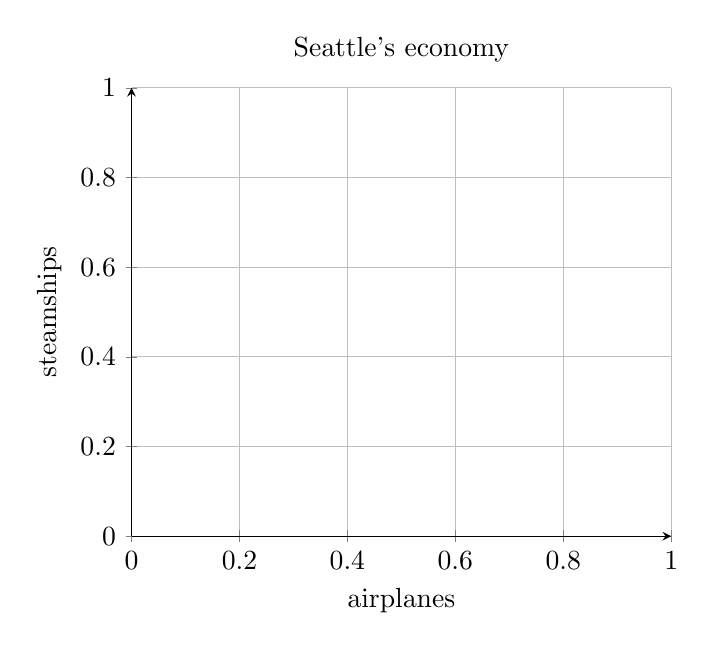
\begin{tikzpicture}
\begin{axis}[grid=both,
  axis y line=left,axis x line=bottom,
  xlabel={airplanes},
  ylabel={steamships},
  title={Seattle's economy}]
    \node[label={45:{$A$}},circle,fill,inner sep=2pt] at (axis cs:0,1) {};
    \node[label={45:{$B$}},circle,fill,inner sep=2pt] at (axis cs:2,2) {};
    \node[label={45:{$C$}},circle,fill,inner sep=2pt] at (axis cs:4,0) {};
\end{axis}
\end{tikzpicture}

\end{document}